\documentclass{howto}
% \usepackage{distutils}
\usepackage{palatino}
\renewcommand{\ttdefault}{cmtt}
\renewcommand{\sfdefault}{cmss}
\newcommand{\myhdl}{\protect \mbox{MyHDL}}
\usepackage{graphicx}
% $Id$

\title{What's New in \myhdl\ 0.3}
\release{0.3}
\author{Jan Decaluwe}
\authoraddress{\email{jan@jandecaluwe.com}}

\begin{document}
\maketitle
\tableofcontents


\section{VCD output for waveform viewing\label{section-wave}}

\ifpdf
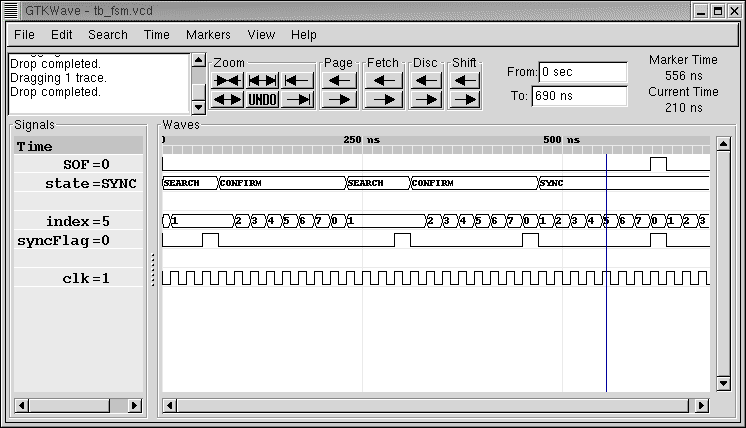
\includegraphics{tbfsm.png}
\fi

\myhdl\ now has support for waveform viewing. During simulation, signal
changes can be written to a VCD output file.  The VCD file can then be
loaded and viewed in a waveform viewer tool such as \program{gtkwave}.

The user interface of this feature consists of a single function,
\function{trace_sigs()}.  To explain how it works, recall that in
\myhdl{}, an instance is created by calling a function that returns a
sequence of generators. For example:

\begin{verbatim}
tb_fsm = testbench()
\end{verbatim}

The \code{tb_fsm} instance is subsequently passed 
as an argument to a \class{Simulation} object constructor
for simulation. To enable VCD tracing, the instance should 
be created as follows instead:

\begin{verbatim}
tb_fsm = trace_sigs(testbench)
\end{verbatim}

As a result, all signals in the instance hierarchy will be traced in
an output VCD file called \file{tb_fsm.vcd}. Note that the argument of
\function{trace_sigs()} consists of the uncalled function. By calling
the function under its control, \function{trace_sigs()} gathers
information about the hierarchy and the signals to be traced.  In
addition to a function argument, \function{trace_sigs()} accepts an
arbitrary number of non-keyword and keyword arguments that will be
passed to the function call.

The restrictions on VCD tracing are as follows. First, only
\class{Signal} objects can be traced. Second, only a hierarchy of
instances returned by a pre-simulation top level function call can be
traced. Also, all instances to be traced should have a name: this is
done by assigning the result of an instantiating function call to a
local variable (instead of using it directly.)

Signals are dumped in a suitable format. This format is inferred at
the \class{Signal} construction time, from the type of the initial
value. In particular, \class{bool} signals are dumped as single
bits. (This only works starting with Python2.3, when \class{bool} has
become a separate type).  Likewise, \class{intbv} signals with a
defined bit width are dumped as bit vectors. To support the general
case, other types of signals are dumped as a string representation, as
returned by the standard \function{str()} function.

\section{An enumeration type\label{section-enum}}

It is often desirable to define a set of identifiers.  A standard
Python idiom is to assign a range of integers to a tuple of
identifiers, like so:

\begin{verbatim}
>>> SEARCH, CONFIRM, SYNC = range(3)
>>> CONFIRM
1
\end{verbatim}

This technique is perfectly acceptable and can be used to write
clearer code. However, there are some drawbacks. Though it is clearly
the intention that the identifiers belong together, this information
is lost as soon as they are defined. Also, the identifiers evaluate to
integers, whereas a string representation of the identifiers
would be preferable. To solve these issues, we need an
\emph{enumeration type}.

\myhdl\ 0.3 supports enumeration types by providing a function
\function{enum()}.  The arguments to \function{enum()} are the string
representations of the identifiers, and its return value is an
enumeration type. The identifiers are available as attributes of the
type. For example:

\begin{verbatim}
>>> from myhdl import enum
>>> t_State = enum('SEARCH', 'CONFIRM', 'SYNC')
>>> t_State
<Enum: SEARCH, CONFIRM, SYNC>
>>> t_State.CONFIRM
CONFIRM
\end{verbatim}

Enumeration types are often used for the state variable in a finite
state machine.  In the waveform in Section~\ref{section-wave}, you see
a \class{Signal} called \code{state} which as been constructed with an
enumeration type identifier as initial value, as follows:

\begin{verbatim}
state = Signal(t_State.SEARCH)
\end{verbatim}

Note that the waveforms show the string representation of the
enumeration type identifiers. 

\section{Inferring the sensitivity list for combinatorial logic}

\section{Inferring the list of all instances\label{section-instances}}

In \myhdl{}, the instances defined in a top level function
need to be returned explicitly, according
the following template:

\begin{verbatim}
def top(...):
    ...
    instance_1 = module_1(...)
    instance_2 = module_2(...)
    ...
    instance_n = module_n(...)
    ... 
    return instance_1, instance_2, ... , instance_n
\end{verbatim}


This permits fine grained control: for example, it
is possible to return a different set of instances
under parameter control. 

However, having to return instances explicitly can be inconvenient,
expecially if there are a large number of them. Therefore, \myhdl\ 0.3
provides a function \function{instances()} which assembles a list of
all instances automatically. It is used as follows:

\begin{verbatim}
from myhdl import instances

def top(...):
    ...
    instance_1 = module_1(...)
    instance_2 = module_2(...)
    ...
    instance_n = module_n(...)
    ...
    return instances()
\end{verbatim}

Function \function{instances()} uses introspection to
inspect the local variables defined by the calling
function. In \myhdl {}, an instance is defined as
a nested sequence of generators: all such variables
are looked up and assembled in a list.

\section{Inferring the list of all processes\label{section-processes}}

In addition to instances, a top level function may
also define local generators functions, which I will
call \emph{processes} because of the analogy with VHDL.
Like instances, processes need to be returned explicitly,
with the qualification that they have to be called first
to turn them into generators. The template is as follows:

\begin{verbatim}
def top(...):
    ...
    def process_1():
        ...
        yield ...
        ...
    def process_2():
        ...
        yield ...
        ...
    def process_n():
        ...
        yield ...
        ...
    ...
    return process_1(), process_2(), ..., process_n()
\end{verbatim}

As for instances, it may be more convenient to assemble the list of
processes automatically. One option is to turn each process into an
instance by calling it and assigning the returned generator to a
local variable. Those instances will then be found by the
\function{instances()} function described in
Section~\ref{section-instances}.

Another option is to use the function \function{processes()} provided
by \myhdl\ 0.3 . This function uses introspection to find the
processes, calls each of them, and assembles the returned generators
into a list. It can be used as follows:

\begin{verbatim}
def top(...):
    ...
    def process_1():
        ...
        yield ...
        ...
    def process_2():
        ...
        yield ...
        ...
    def process_n():
        ...
        yield ...
        ...
    ... 
    return processes()
\end{verbatim}

To conclude, a top level function with both instances and
processes can use the following idiomatic code to
return all of them:

\begin{verbatim}
return instances(), processes()
\end{verbatim}


\section{Python 2.3 support\label{section-Python}}

As of this writing, Python 2.3 is the latest Python release.  \myhdl\
0.3 works with both Python 2.2 and Python 2.3. In good Python
tradition, \myhdl\ code developed with Python2.2 will run without
changes or problems in Python 2.3.

In general, I am not that keen on fast upgrading. However, as it
happens, the evolution of Python enables features that are really
important or even crucial to \myhdl{}.  Python 2.2 generators are the
best example: they are the cornerstone of \myhdl{}. But Python 2.3
also has significant benefits, which I will summarize below.

First, generators and the \code{yield} statement are a default Python
2.3 feature. This means that \code{from __future__ import generators}
statements are no longer required.

Second, Python 2.3 has a \class{bool} type, which is implemented as a
subtype of \class{int}. For general Python use, the implications are
rather limited - the main difference is that logical result values will
print as \code{False} and \code{True} instead of \code{0} and
\code{1}. However, in \myhdl{}, I can use the \class{bool} type to infer
a bit width.  If a \class{Signal} is constructed with a \class{bool}
value, it is a single bit \class{Signal}. One application is waveform
viewing as in Section~\ref{section-wave}. In the waveform, note how
single bit signals are displayed as level changes.  With Python 2.2,
the waveforms of these signals would only show value changes,
which is not as clear for single bits.

Finally, Python 2.3 is significantly faster. \myhdl\ code runs
25--35\% faster in Python 2.3 - a nice speedup.

Python is a very stable language, so upgrading to Python 2.3 is
virtually risk free. Given the additional benefits, I recommend
\myhdl\ users to do so as soon as possible. For the next major release
(0.4), the new features will become crucial and only Python 2.3 (and
higher) will be supported.


\end{document}
